%%%%%%%%%%%%%%%%%%%%%%%%%%%%%%%%%%%%%%%%%%%%%%%%%%%%%%%%%%%%%%%%%%%%%%%%%%%%%%%%
%                           RESULTS DATASET CW CHES                          %
%%%%%%%%%%%%%%%%%%%%%%%%%%%%%%%%%%%%%%%%%%%%%%%%%%%%%%%%%%%%%%%%%%%%%%%%%%%%%%%%
\begin{figure}
    \centering
    \begin{subfigure}{0.49\textwidth}
        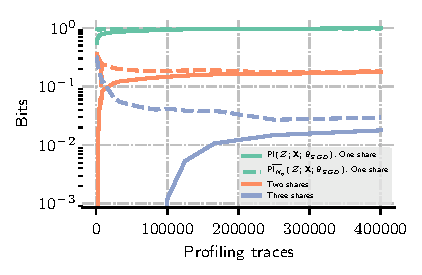
\includegraphics{Figures/experiments/learning_curves_05}
        \caption{Learning curve of Experiment 4 on Boolean secret-sharing.}
        \label{fig:exp_PI_4}
    \end{subfigure}
    \begin{subfigure}{0.49\textwidth}
        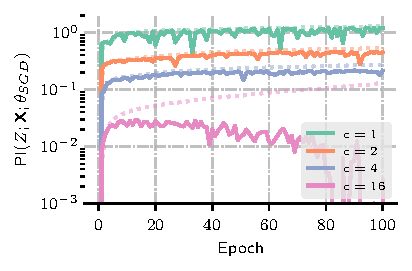
\includegraphics{Figures/experiments/PI_shuffle_4_bits}
        \caption{Results of Experiment 5 on shuffling.}
        \label{fig:exp_PI_5}
    \end{subfigure}
    \caption{Results on experimental data.}
    \label{fig:exp_PI}
\end{figure}
\autoref{fig:exp_PI_4} presents the learning curves of Experiment 4, when targeting respectively \(1, 2\) or \(3\) shares among the considered ones.
The dotted curves are the estimated \gls{pi} over the \(\numTracesProf = \card{\trainSet}\) profiling traces whereas the plain curves denote the \gls{pi} estimated with the \(\numTracesVal\) validation traces.
  
It may first be observed that the amount of information leaking on the sensitive un-split variable seems to decrease at an exponential rate in the number of shares, as expected from both theory -- see \autoref{sec:masking} -- and our simulations -- see \autoref{sec:simus}.
More interestingly, the gap between dotted curves and their corresponding plain ones exactly corresponds to the estimation error term~\eqref{eq:err_est_ches}.
It appears then that the latter one becomes negligible relatively to the \gls{pi} when the profiling set size exceeds respectively a few thousands when targeting one share, or one hundred thousand when targeting two shares.
When targeting three shares, the estimation error is not completely negligible, even with \(400,000\) profiling traces.
It is furthermore particularly noticeable that when profiling the three shares scheme with less than \(100,000\) traces, the learning phase completely failed since the \gls{pi} was null. 
This indicates that, in addition to the effect on \gls{mi} predicted by theoretical works, the secret-sharing counter-measure also has an effect on the \gls{pi} through an increasing estimation error, making the \gls{mi} estimation poorer.
  
  
\autoref{fig:exp_PI_5} presents the results of Experiment 5 on shuffling. 
It is recalled that contrary to Experiment 4 where \glspl{poi} where extracted, here \(250\)-dimensional traces have been processed through a \gls{dnn}. 
The gap in \autoref{fig:exp_MI_3} between each curve remains observable on \autoref{fig:exp_PI_5} when considering experimental traces.
However, the \gls{pi} obtained when the attack target is shuffled among \(16\) random values seems decreasing starting the \(20\)-th epoch, while the empirical \gls{pi} (in dotted curves) keeps increasing.
This is a sign of \emph{over-fitting}.

% Over-fitting
Indeed, if the estimation error is high, the optimization algorithm is expected to return at each iteration a better model with respect to the training loss \(\LossFunc[\trainSet]{}\).
Since the latter one is different from the cross entropy \(\LossFunc[\XXX, \Z]{}\), an improvement with respect to the training loss may not be an improvement with respect to the cross entropy, or equivalently, with respect to the \gls{pi}.
That is why there is a moment when the loss computed over the validation traces starts increasing whereas the training loss keep decreasing.
In other words, the model starts to learn \emph{by heart} to build its prediction on some uninformative features which would not generalize well during the attack phase on unknown traces.
The higher the estimation error, the less similar the \gls{nll} loss and the cross entropy so the sooner and the more importantly over-fitting happens.
Therefore, the \gls{pi} reached in the graph is not necessarily optimal: more profiling traces might be required to decrease the estimation error and thereby mitigating the effect of over-fitting.

Altogether, our experiments show that similarly to the approximation and optimization errors discussed in \autoref{sec:simus}, the estimation error is also negligible relatively to the \gls{mi}, when considering unprotected scenarios where the profiling set size is reasonably high (\ie{} \(10,000\) traces or above). 
This therefore leads to a tight estimation of the \gls{mi} through the maximization of the \gls{pi} (\ie{} the minimization of the \gls{nll} loss).
When considering protected devices, the investigated counter-measures impact the estimation error, and thereby the tightness of the lower bound computed through \gls{pi} maximization.
Nevertheless this can be controlled by increasing the size of the profiling set.
More precisely, the \textit{harder} the counter-measure (\ie{} the higher the sharing order, or the more shuffled bytes), the higher the profiling set size.
  
  
Another way to decrease the estimation error would be to decrease the \textit{capacity} of the hypotheses class, \ie{} its \gls{vc}-dimension, by decreasing the number of layers or the number of neurons on each layer. 
Since we have argued in \autoref{sec:analysis_simus} that the approximation error was negligible even for a simple architecture, we are quite confident that this would not strongly affect the quality of the \gls{mi} estimation.